\documentclass[11pt, a4paper]{article}

%-------------------------------------------------------------------------------
% Lingua E Codifica
%-------------------------------------------------------------------------------
\usepackage[italian]{babel}
\usepackage[utf8]{inputenc}
\usepackage[T1]{fontenc}

%-------------------------------------------------------------------------------
% Layout Di Pagina E Tipografia
%-------------------------------------------------------------------------------
\usepackage[margin=2cm, top=1.5cm, bottom=1.5cm]{geometry}
\usepackage{parskip}
\usepackage[expansion=false]{microtype}

%-------------------------------------------------------------------------------
% Gestione Dei Colori
%-------------------------------------------------------------------------------
\usepackage[table]{xcolor}

%-------------------------------------------------------------------------------
% Matematica E Simboli
%-------------------------------------------------------------------------------
\usepackage{amsmath, amssymb, amsfonts}
\usepackage{mathtools}
\usepackage{siunitx}

% BB OTTIMIZZAZIONE MATRICI LUNGHE PER LA STAMPA
\setlength{\arraycolsep}{10pt}
\usepackage{bm}

%-------------------------------------------------------------------------------
% Grafica, Immagini E Tabelle
%-------------------------------------------------------------------------------
\usepackage{graphicx}
\graphicspath{{./Images/Appunti}}
\usepackage{float}
\usepackage{booktabs}
\usepackage{array}
\usepackage{multirow}
\usepackage{tabularx}
\usepackage{listings}
\usepackage{tikz}
\usetikzlibrary{shapes.geometric, arrows.meta, positioning, calc, quotes}

%-------------------------------------------------------------------------------
% Link, Riferimenti Ed Elenchi
%-------------------------------------------------------------------------------
\usepackage[unicode]{hyperref}
\hypersetup{
    colorlinks=true,
    linkcolor=blue,
    urlcolor=blue,
    citecolor=blue,
    pdftitle={Capitolo 1},
    pdfauthor={Francesco Lo Verde},
    pdfpagemode=FullScreen,
}
\usepackage{bookmark}
\usepackage[italian,capitalize]{cleveref}
\usepackage{enumitem}
\setlist{noitemsep}

%-------------------------------------------------------------------------------
% Personalizzazione Titoli E Altri Pacchetti
%-------------------------------------------------------------------------------
\usepackage{titlesec}
\titleformat{\section}{\normalfont\LARGE\bfseries}{\thesection}{1em}{}
\titleformat{\subsection}{\normalfont\Large\bfseries}{\thesubsection}{1em}{}
\titleformat{\subsubsection}{\normalfont\large\bfseries}{\thesubsubsection}{1em}{}

\usepackage{comment}
\newtheorem{theorem}{Definizione}

\author{Francesco Lo Verde}
\begin{document}

\section{Introduzione}
Un robot è costituito da un sistema meccanico che include organi di locomozione, come ruote, cingoli o gambe meccaniche, e organi di manipolazione, quali bracci meccanici, mani artificiali e utensili.

\begin{figure}[h]
    \centering
    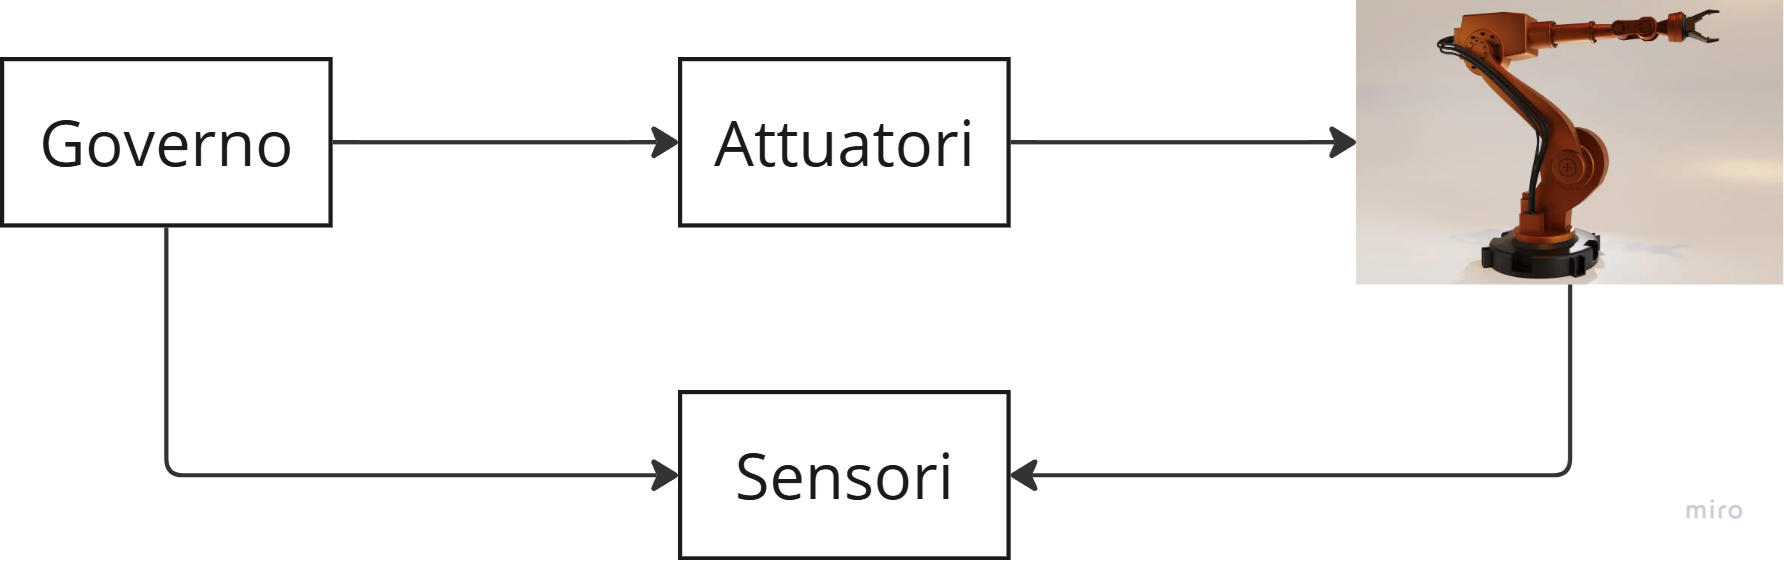
\includegraphics[width=0.75\linewidth]{Schema.png}
\end{figure}

L'animazione delle componenti meccaniche è garantita da un sistema di attuazione, che include servomotori, azionamenti e organi di trasmissione. La percezione dell'ambiente è affidata a un sistema sensoriale composto da sensori propriocettivi (trasduttori di posizione) e sensori esterocettivi (sensori di forza, telecamere). Infine, il sistema di governo integra azione e percezione, comandando l'esecuzione delle operazioni nel rispetto di obiettivi e vincoli.
\begin{theorem}
    \textbf{ISO 8373}\\
    Un robot è un sistema meccanico programmabile, dotato di un certo grado di autonomia, capace di eseguire compiti fisici in ambienti strutturati o non strutturati.
\end{theorem}

\begin{theorem}
    \textbf{IFR}\\
    Un robot industriale è un manipolatore multifunzionale, programmabile in tre o più assi, capace di muoversi autonomamente per eseguire compiti specifici di manipolazione o assemblaggio.
\end{theorem}

\begin{theorem}
    \textbf{Robot Istitute Of America} (Libro)\\
    Un robot e una struttura meccanica multifunzionale e riprogrammabile progettato per spostare materiali, parti, utensili o dispositivi specializzati secondo movimenti variabili programmati per l’esecuzione di una varieta di compiti diversi.
\end{theorem}
\newpage
\section{Struttura Meccanica dei Robot}
I robot si distinguono in due categorie principali: \textbf{robot a base fissa}, detti manipolatori, e \textbf{robot mobili}.

\subsection{Robot A Base Fissa (Manipolatori)}
La struttura meccanica di un robot manipolatore consiste in un insieme di corpi ridigi (\textit{bracci}) interconnessi tra di loro per mezzo di articolazioni (\textit{giunti}); nel manipolatore si individuano una struttura portante, che ne assicura mobilità, un
\textit{polso}, che conferisce destrezza, e un \textit{organo terminale} che esegue il compito per cui il robot è utilizzato.\\
\textbf{La struttura fondamentale dei manipolatori è a catena cinematica aperta o seriale}

Dal punto di vista topologico, si distinguono:
\begin{itemize}
	\item \textbf{Catene Cinematiche Aperte}, in cui una sequenza unica di bracci collega gli estremi della catena.
	\item \textbf{Catene Cinematiche Chiuse}, in cui una sequenza di bracci forma un anello, riducendo i gradi di libertà a causa dei vincoli imposti.
\end{itemize}
La mobilità di un manipolatore `e assicurata dalla presenza dei giunti. L'articolazione tra due bracci consecutivi può essere realizzata con un giunto \textbf{prismatico} o \textbf{rotoidale}. Un giunto \textit{prismatico} permette traslazione tra due bracci, mentre un giunto \textit{rotoidale} consente la rotazione. La scelta tra queste soluzioni dipende da esigenze di compattezza e affidabilità.
In una catena cinematica aperta, ogni giunto (di entrambi i tipi) conferisce un singolo grado di libertà (DoF) e quindi questi dipendono dalla configurazione dei giunti.\\
I gradi di libertà devono essere opportunamente distribuiti lungo la struttura
meccanica in modo da essere in numero sufficiente per l'esecuzione di un dato
compito. Per operazioni tridimensionali, sono necessari almeno sei gradi di libertà (tre per la posizione e tre per l'orientamento). Un manipolatore con più DoF di quelli strettamente necessari è detto \textbf{ridondante}.\\
Lo \textit{spazio di lavoro} rappresenta la porzione dell'ambiente circostante a cui
può accedere l'organo terminale di un manipolatore. La sua forma e il suo volume
dipendono dalla struttura del manipolatore.
\newpage
\subsubsection{Tipologie di Manipolatori}
Il compito della \textit{struttura portante} è quello di posizionare il polso che orienterà l'organo terminale. Il tipo e la successione dei gradi di libertà della struttura portante, a partire dall'articolazione alla base, consente di classificare i manipolatori in:
\begin{itemize}
	\item \textbf{Manipolatori cartesiani}: Basati su tre giunti prismatici ortogonali, consentono movimenti rettilinei e alta precisione su tutto il volume di lavoro. Ad ogni grado di libertà corrispomde una variabile dello spazio cartesiano e quindi si possono immediatamente definire percorsi rettilinei. La precisione di posizionamento del polso è costante in tutto lo spazio. Lo spazio di lavoro è un parallelepipedo

	\item \textbf{Manipolatori cilindrici}: Presentano un giunto rotoidale alla base e due giunti prismatici. Descrivendo il compito in coordinate cilindriche ogni grado di libertà corrisponde ad una variabile dello spazio. La precisione di posizionamento del polso si riduce al crescere dello sbraccio orizzontale. Lo spazio di lavoro è una porzione di cilindro cavo

	\item \textbf{Manipolatori sferici}: con due giunti rotoidali (primo e secondo) e uno prismatico, permettono l'accesso a un ampio spazio di lavoro sferico, ma con minore rigidezza strutturale. Descrivendo il compito in coordinate sferiche ogni grado di libertà corrisponde ad una variabile dello spazio. La precisione di posizionamento del polso si riduce al crescere dello sbraccio radiale. Lo spazio di lavoro è una porzione di sfera cava


	\item \textbf{SCARA (Selective Compliance Assembly Robot Arm)}: Dotati di due giunti rotoidali e un prismatico, posizionati in modo tale che gli assi siano tutti paralleli tra di loro. Descrivendo il compito in coordinate cartesiane, la corrispondenza tra gradi di libertà e variabili dello spazio cartesiano è mantenuta solo per la componente verticale. La precisione di posizionamento del polso si riduce al crescere della distanza del polso dall'asse del primo giunto

	\item \textbf{Manipolatori antropomorfi}: Composti da tre giunti rotoidali (spalla, gomito e polso), simulano la mobilità del braccio umano, garantendo elevata destrezza. L'asse di rotazione del giunto di base è ortogonale agli altri due che sono paralleli tra loro. Si si perde del tutto la corrispondenza tra gradi di libertà e variabili dello spazio cartesiano, nonché la precisione di posizionamento del polso cambia in tutto lo spazio di lavoro

	\item \textbf{Manipolatori paralleli}: Caratterizzati da catene cinematiche chiuse, che connettono la base all'organo terminale. Il vantaggio è l'elevata rigidezza strutturale rispetto ai manipolatori a catena cinematica aperta
\end{itemize}

\subsubsection{Il Polso e l'Organo Terminale}
Per garantire orientamenti arbitrari in uno spazio tridimensionale, il polso deve possedere \textit{almeno tre gradi di libertà}, realizzati mediante giunti rotoidali. Questi giunti consentono movimenti indipendenti attorno a tre assi, permettendo al manipolatore di raggiungere qualsiasi orientamento desiderato. Tuttavia, poiché il polso costituisce la parte terminale del manipolatore, deve soddisfare requisiti di compattezza che spesso complicano il suo progetto meccanico.\\
La soluzione più efficace consiste è quella in cui i tre assi di rotazione si intersecano in un unico punto e questa configurazione è detta \textbf{Polso Sferico}. La caratteristica principale è il disaccoppiamento tra posizione e orientamento dell'organo terminale. In altre parole, la struttura portante del manipolatore è responsabile di posizionare il punto di intersezione degli assi del polso, mentre il polso stesso si occupa di determinare l'orientamento finale dell'organo terminale. Tale separazione semplifica notevolmente il coordinamento tra i movimenti della struttura portante e quelli del polso.\\
L'organo terminale di un manipolatore è scelto in base al compito specifico che il robot deve eseguire. Ad esempio, per compiti di trasporto, l'organo terminale è generalmente costituito da una pinza, per applicazioni di lavorazione o assemblaggio, invece, l'organo terminale può essere un utensile specializzato, come una torcia di saldatura, una fresa, un trapano o un avvitatore.

Un esempio pratico è rappresentato dai robot utilizzati nell'industria automobilistica, dove manipolatori dotati di torce di saldatura eseguono operazioni di giunzione su componenti metallici. In questo caso, la precisione del posizionamento e la capacità del polso di orientare correttamente la torcia sono fattori critici per garantire la qualità del risultato.

% La versatilità e la flessibilità dei robot manipolatori non devono indurre a pensare che tutte le strutture meccaniche siano equivalenti per l'esecuzione di un determinato compito. La scelta di un robot è infatti condizionata dall'applicazione specifica, che impone vincoli riguardanti:
% \begin{itemize}
%     \item \textbf{Dimensione e forma dello spazio di lavoro}: Il manipolatore deve essere in grado di raggiungere tutti i punti rilevanti per il compito.
%     \item \textbf{Portata di carico}: Il robot deve supportare il peso dell'organo terminale e dell'eventuale carico manipolato.
%     \item \textbf{Destrezza}: La capacità del polso di eseguire orientamenti complessi è essenziale per compiti che richiedono alta precisione.
%     \item \textbf{Precisione di posizionamento}: Errori minimi possono compromettere la qualità del risultato, soprattutto in applicazioni critiche come l'assemblaggio di componenti elettronici.
%     \item \textbf{Prestazioni dinamiche}: Velocità e accelerazione del manipolatore influenzano l'efficienza del processo produttivo.
% \end{itemize}

\newpage
\subsection{Robot Mobili}
I robot mobili sono caratterizzati dalla presenza di una base semovente che consente loro di spostarsi autonomamente nell'ambiente in cui operano. A differenza dei manipolatori, questi robot sono impiegati principalmente in applicazioni di servizio, dove un'elevata mobilità è un requisito essenziale. Da un punto di vista meccanico, un robot mobile è costituito da uno o più corpi rigidi dotati di un sistema di locomozione. In generale, si distinguono due categorie principali:


\begin{itemize}
    \item \textbf{Robot Mobili Su Ruote}: Questi robot presentano un corpo rigido (chassis) equipaggiato con ruote per la locomozione. In alcuni casi, possono essere collegati ad altri corpi rigidi (rimorchi) tramite giunti rotoidali, anch'essi dotati di ruote.
    \item \textbf{Robot Mobili Su Gambe}: Questa categoria include robot con più corpi rigidi connessi tra loro mediante giunti prismatici o rotoidali. Alcuni di questi corpi formano arti, le cui estremità (piedi) entrano periodicamente in contatto con il suolo per realizzare il movimento. La varietà di strutture è vasta e spesso si ispira alla biomeccanica degli organismi viventi (robotica biomimetica), spaziando dai robot bipedi umanoidi ai robot esapodi che emulano il movimento degli insetti.
\end{itemize}

Le ruote convenzionali si suddividono in tre categorie:
\begin{itemize}
    \item \textbf{Ruota Fissa}: ruota attorno a un asse passante per il suo centro e normale al piano, mantenendo un orientamento costante rispetto allo chassis.

    \item \textbf{Ruota Orientabile}: presenta due assi di rotazione: uno uguale a quello della ruota fissa per la rotazione e uno verticale che ne consente l'orientamento rispetto allo chassis.

    \item \textbf{Ruota Eccentrica (Caster)}: simile alla ruota orientabile, ma con l'asse verticale spostato rispetto al centro della ruota. Questa configurazione permette alla ruota di allinearsi automaticamente alla direzione di spostamento dello chassis, senza influenzarne la mobilità.
\end{itemize}

I robot mobili possono adottare diverse configurazioni di trazione, tra cui:
\begin{itemize}
    \item \textbf{Trazione Differenziale}: Questa configurazione prevede due ruote fisse con un asse di rotazione comune e una o più ruote eccentriche per il bilanciamento statico. Il robot può ruotare sul posto se le velocità angolari delle due ruote principali sono uguali e opposte.

    \item \textbf{Trazione Sincronizzata}: Un robot con questa configurazione possiede tre ruote orientabili allineate, controllate da due motori: uno per la trazione e uno per l'orientamento.

    \item \textbf{Configurazione Triciclo}: Comprende due ruote fisse posteriori e una ruota orientabile anteriore. La trazione è fornita da un unico motore per le ruote fisse, mentre un secondo motore controlla l'orientamento della ruota anteriore e quindi agisce da sterzo.

    \item \textbf{Configurazione Automobilistica}: Presenta due ruote fisse posteriori e due ruote orientabili anteriori. Un motore fornisce la trazione, mentre un altro gestisce l'orientamento delle ruote anteriori. Per evitare slittamenti in curva, le ruote anteriori assumono angoli di sterzata differenti: la ruota interna è più sterzata rispetto a quella esterna. A differenza dei precedenti, questo veicolo è \textit{omnidirezionale}, cioè può muoversi istantaneamente in qualsiasi direzione
\end{itemize}

% Oltre alle ruote convenzionali, esistono ruote speciali come la \textbf{ruota Mecanum} (o svedese), dotata di rulli passivi inclinati (solitamente di $45^{\circ}$), che permettono una mobilità omnidirezionale.

\subsubsection{Bilanciamento e Stabilità}
Nel caso dei robot mobili su ruote, il bilanciamento non costituisce generalmente un problema. Un robot con tre ruote è in equilibrio statico se il baricentro si trova all'interno del triangolo di supporto formato dai punti di contatto delle ruote con il suolo. Nei robot con più di tre ruote, il poligono di supporto garantisce maggiore stabilità, ma in presenza di superfici irregolari è necessario un sistema di sospensioni per mantenere il contatto con il suolo.\\
A differenza dei manipolatori, lo spazio di lavoro di un robot mobile può essere potenzialmente illimitato. Tuttavia, un robot non omnidirezionale presenta restrizioni sui moti istantanei ammissibili. Ad esempio, un robot a triciclo non può muoversi immediatamente in direzione perpendicolare all'asse delle ruote posteriori, sebbene sia comunque in grado di raggiungere tale posizione attraverso manovre appropriate. In generale, le limitazioni istantanee non precludono la possibilità di raggiungere qualsiasi posizione e orientamento all'interno dello spazio di lavoro.

\newpage
\subsection{Robotica Industriale}

La robotica industriale si occupa della progettazione, del controllo e delle applicazioni dei robot in ambito produttivo. I robot industriali operano in ambienti strutturati, le cui caratteristiche geometriche e fisiche sono note a priori. Grazie agli sviluppi tecnologici, questa disciplina ha raggiunto un alto grado di maturità, diventando un pilastro dell'automazione moderna.

L'automazione industriale ha l'obiettivo di sostituire l'uomo in un processo produttivo, non solo nell'esecuzione delle operazioni materiali, ma anche nell'elaborazione intelligente delle informazioni sullo stato del processo. A seconda della flessibilità del sistema, si distinguono tre principali tipologie di automazione:

\begin{itemize}
    \item \textbf{Automazione Rigida}: Impiegata in contesti produttivi caratterizzati da elevati volumi di produzione di manufatti con caratteristiche costanti. In questi scenari, la necessità di garantire alta produttività e qualità impone l'uso di macchinari specializzati e sequenze operative prestabilite. Questo tipo di automazione è tipico delle catene di montaggio, in cui la ripetitività e l'efficienza sono prioritarie.
    \item \textbf{Automazione Programmabile}: Adottata in ambienti di produzione orientati alla realizzazione di piccoli e medi lotti di prodotti con caratteristiche variabili. Un sistema di automazione programmabile consente di modificare le sequenze operative attraverso la riprogrammazione dei macchinari, permettendo una maggiore adattabilità alle esigenze produttive. Questo approccio è tipico di industrie che devono rispondere a una domanda diversificata, come quelle del settore automobilistico e dell'elettronica.
    \item \textbf{Automazione Flessibile}: Rappresenta l'evoluzione dell'automazione programmabile, consentendo la produzione di lotti variabili con un'efficienza superiore. Il suo obiettivo è minimizzare i tempi di inattività necessari per la riprogrammazione delle operazioni e delle macchine impiegate. Tale automazione si basa su sistemi di controllo avanzati e robot industriali dotati di sensori e algoritmi di apprendimento automatico, che li rendono in grado di adattarsi dinamicamente alle variazioni della produzione.
\end{itemize}

Un robot industriale possiede tre capacità fondamentali che lo rendono essenziale nei processi manifatturieri:

\begin{itemize}
    \item \textbf{Trasporto}: Movimentazione di componenti e prodotti all'interno della
    linea di produzione;
    \item \textbf{Manipolazione}: Esecuzione di operazioni di assemblaggio, saldatura, verniciatura e altre attività che richiedono precisione;
    \item \textbf{Misura}: Acquisizione di dati relativi alla qualità del prodotto e alle condizioni operative, permettendo il controllo e l'ottimizzazione del processo.
\end{itemize}

\newpage
\section{Modellistica, Pianificazione, E Controllo Di Robot}
In tutte le applicazioni robotiche, l'esecuzione di un compito richiede l'implementazione di un movimento pianificato. La corretta realizzazione di tale movimento dipende dall'unità di governo, la quale fornisce i comandi necessari agli attuatori del robot. Per garantire un'esecuzione precisa, è essenziale un'analisi approfondita della struttura meccanica, degli attuatori e dei sensori.
L'obiettivo di questa analisi è la derivazione di modelli matematici capaci di descrivere i legami tra i vari componenti del robot, fornendo così una base indispensabile per la progettazione delle strategie di controllo del movimento.

\subsection{Modellistica}
L'analisi cinematica di un robot si occupa della descrizione del moto rispetto a un sistema di riferimento cartesiano fisso, senza considerare le forze e i momenti che lo generano.
Essa si distingue in cinematica diretta e inversa:
\begin{itemize}
    \item \textbf{Cinematica Diretta}: Determina la posizione e l'orientamento dell'organo terminale a partire dalle coordinate dei giunti.
    \item \textbf{Cinematica Inversa}: Consente di calcolare i moti dei giunti necessari per raggiungere una specifica posizione e orientamento dell'organo terminale.
\end{itemize}

La cinematica differenziale, tramite lo Jacobiano del manipolatore, descrive le relazioni tra le velocità dei giunti e quelle dell'organo terminale. Essa costituisce la base per derivare il modello dinamico del robot, che esprime le equazioni del moto in funzione delle forze e dei momenti applicati. Un modello dinamico accurato è essenziale per dimensionare gli attuatori, progettare strategie di controllo e simulare il comportamento del sistema.

Nel caso dei robot mobili, la modellistica si differenzia da quella dei manipolatori per la presenza di vincoli cinematici legati alle ruote. Tali vincoli, integrabili o meno a seconda della struttura meccanica, influenzano direttamente la mobilità del robot. Il modello cinematico descrive i moti istantanei ammissibili sotto tali vincoli, mentre il modello dinamico, che include le reazioni vincolari, lega questi moti alle forze generalizzate agenti sul sistema.

\subsection{Pianificazione Del Movimento}
La pianificazione del moto definisce il movimento da imporre ai giunti o direttamente all'organo terminale. Si distinguono due principali approcci:
\begin{itemize}
    \item \textbf{Moto Punto-Punto}: Utilizzato in operazioni di trasporto, in cui è sufficiente definire le posizioni di partenza e di arrivo.
    \item \textbf{Moto Su Percorso Assegnato}: Impiegato in lavorazioni, dove l'organo terminale deve seguire una traiettoria specifica.
\end{itemize}
Il problema di pianificazione nei robot mobili consiste nel generare traiettorie che conducano il veicolo da una configurazione iniziale a una finale. Se lo spazio di lavoro contiene ostacoli, la pianificazione deve garantire l'assenza di collisioni.Tale problema, noto come \textit{pianificazione del moto}, si può formulare in modo valido tanto per i manipolatori quanto per i robot mobili utilizzando il concetto di spazio delle configurazioni.

\newpage

\subsection{Controllo del Movimento}
Il controllo di un robot richiede l'uso di attuatori e sensori per garantire l'esecuzione delle traiettorie pianificate, che costituiscono gli ingressi di riferimento per il sistema di controllo. Il problema principale nel controllo di un manipolatore è determinare le forze e le coppie che gli attuatori devono applicare ai giunti per seguire tali traiettorie. Questo compito è complesso poiché i manipolatori sono sistemi articolati in cui il moto di un braccio influenza quello degli altri. Le equazioni del moto evidenziano, tranne nel caso di strutture cartesiane ad assi ortogonali, accoppiamenti dinamici tra i giunti. La sintesi delle forze e coppie non può basarsi solo sul modello dinamico, poiché esso non descrive completamente la struttura reale. Pertanto, il controllo si affida alla retroazione: valutando lo scostamento tra i riferimenti e le misure dei sensori propriocettivi, un sistema in retroazione soddisfa le specifiche di precisione richieste.

Il controllo di un robot mobile differisce sostanzialmente da quello dei manipolatori. In questo caso, il numero di ingressi di controllo è sempre inferiore al numero di variabili di configurazione. Di conseguenza, la struttura di un controllore per l'inseguimento di traiettorie è necessariamente diversa da quella di un controllore per raggiungere una configurazione specifica.

\end{document}
